\section{Уравнения в частных производных}

\subsection{Волновые уравнения (колебания струны)}

Рассмотрим тонкую упругую нить (струну) длины $l$, закрепленную с двух концов, которая может свободно колебаться.

\begin{center}
	\begin{tikzpicture}[scale=1]
		\draw[thick] (0,0) node[below left] {$A$} .. controls (1,1) and (2,-1) .. (3,0.5) .. controls (4,2) and (5,-0.5) .. (6,0) node[below right] {$B$};
		\fill (0,0) circle (2pt);
		\fill (6,0) circle (2pt);
	\end{tikzpicture}
\end{center}

Выделим малый элемент струны $MM'$ проекцией $dx$ на ось $Ox$.

\begin{center}
	\begin{tikzpicture}[scale=1.5]
		\draw[-stealth] (-0.5,0) -- (4,0) node[right] {$x$};
		\draw[-stealth] (0,-0.5) -- (0,3) node[above] {$y$};
		\node[below left] at (0,0) {$0$};
		
		% Curve segment
		\draw[thick, blue] (1,0.5) to[out=20, in=200] (3,2.5);
		
		% Points M and M'
		\coordinate (M) at (1.5, 0.85);
		\coordinate (Mprime) at (2.5, 1.85);
		
		\fill[red] (M) circle (1.5pt) node[above left, black] {$M$};
		\fill[red] (Mprime) circle (1.5pt) node[left, black] {$M'$};
		
		% Projections
		\draw[dashed] (1.5, 0.85) -- (1.5, 0) node[below] {$x$};
		\draw[dashed] (2.5, 1.85) -- (2.5, 0) node[below] {$x+dx$};
		
		% Tangent vectors (Forces)
		\draw[-stealth, red, very thick] (M) -- ($(M) + (-0.8, -0.45)$) node[left] {$\vb{T}_0$};
		\draw[-stealth, red, very thick] (Mprime) -- ($(Mprime) + (0.8, 0.6)$) node[right] {$\vb{T}'_0$};
		
		% Force components diagrams
		\draw[dashed] (M) -- ($(M) + (-0.8, 0)$);
		\draw (M) ++(-0.4,0) arc (180:210:0.4) node[midway, left] {$\alpha$};
		
		\draw[dashed] (Mprime) -- ($(Mprime) + (0.8, 0)$);
		\draw (Mprime) ++(0.4,0) arc (0:36:0.4) node[midway, right] {$\alpha'$};
	\end{tikzpicture}
\end{center}

На выделенный участок $MM'$ действуют силы натяжения со стороны смежных участков струны ($\vb{T}_0$ и $\vb{T}'_0$ соответственно). Будем предполагать, что натяжение струны велико, так что:
\begin{equation}
	|\vb{T}_0| = |\vb{T}'_0| = T_0
\end{equation}

Фиксируем момент времени $t$. Результирующая сила $F$, действующая на элемент в вертикальном направлении:
\begin{equation}
	F = T_0 \sin \alpha' - T_0 \sin \alpha
\end{equation}
Так как углы отклонения малы, можно считать:
\begin{equation}
	\sin \alpha \approx \tan \alpha = \eval{\pdv{u}{x}}_{x} \quad \text{и} \quad \sin \alpha' \approx \tan \alpha' = \eval{\pdv{u}{x}}_{x+dx}
\end{equation}
Следовательно:
\begin{equation}
	F \approx T_0 \qty( \eval{\pdv{u}{x}}_{x+dx} - \eval{\pdv{u}{x}}_{x} ) = T_0 \cdot \Delta \qty(\pdv{u}{x})
\end{equation}

С другой стороны, приращение по вертикальной оси составляет:
\begin{equation}
	\Delta y = y(x+dx) - y(x) \approx y'(x) dx
\end{equation}
Разность первых производных можно приближенно выразить через вторую производную:
\begin{equation}
	\pdv{u}{x}(x+dx, t) - \pdv{u}{x}(x,t) \approx \pdv{x} \qty(\pdv{u}{x}(x,t)) dx = \pdv[2]{u}{x} dx
\end{equation}
Тогда результирующая сила принимает вид:
\begin{equation}
	F \approx T_0 \cdot \pdv[2]{u}{x} dx
\end{equation}

Согласно второму закону Ньютона, сила равна произведению массы элемента струны ($\rho dx$) на его ускорение ($\pdv[2]{u}{t}$):
\begin{equation}
	F = \rho dx \cdot \pdv[2]{u}{t}
\end{equation}
Приравнивая два выражения для силы, получаем:
\begin{equation}
	T_0 \cdot \pdv[2]{u}{x} dx = \rho dx \cdot \pdv[2]{u}{t} \iff \pdv[2]{u}{t} = \frac{T_0}{\rho} \pdv[2]{u}{x}
\end{equation}
Обозначим $a^2 = \frac{T_0}{\rho}$. Тогда получаем \textbf{уравнение свободных колебаний струны}:
\begin{equation}
	\pdv[2]{u}{t} = a^2 \pdv[2]{u}{x}
\end{equation}

Если на струну действуют внешние распределенные силы $F_1$, то уравнение движения записывается в виде:
\begin{equation}
	F + F_1 = \rho dx \cdot \pdv[2]{u}{t}
\end{equation}
\begin{equation}
	a^2 \pdv[2]{u}{x} + \frac{F_1}{\rho dx} = \pdv[2]{u}{t}
\end{equation}
Обозначив $f = \frac{F_1}{\rho dx}$, получаем уравнение для \textbf{вынужденных колебаний}:
\begin{equation}
	\pdv[2]{u}{t} = a^2 \pdv[2]{u}{x} + f
\end{equation}

\subsection{Метод Фурье}

Сформулируем краевую задачу для колебания струны с закрепленными концами:
\begin{equation}
	\begin{cases}
		\pdv[2]{u}{t} = a^2 \pdv[2]{u}{x} \\[1.5ex]
		u(0,t) = u(l,t) = 0 \quad \text{-- граничные условия} \\[1.5ex]
		\begin{aligned}
			u(x,0) &= \varphi(x) \\
			\eval{\pdv{u}{t}}_{t=0} &= \psi(x)
		\end{aligned} \quad \text{-- начальные условия}
	\end{cases}
\end{equation}

\begin{nb}
	Если задано начальное отклонение $\varphi(x)$, то физически это соответствует щипковому инструменту (например, гитаре). Если задана начальная скорость $\psi(x)$ — это ударный музыкальный инструмент (например, фортепиано).
\end{nb}

Ищем нетривиальное решение в виде произведения двух функций, каждая из которых зависит только от одной переменной:
\begin{equation}
	u(x,t) = X(x) \cdot T(t)
\end{equation}
Подставляя этот анзац в исходное уравнение, находим:
\begin{equation}
	X(x) \cdot T''(t) = a^2 X''(x) \cdot T(t) \iff \frac{T''(t)}{a^2 T(t)} = \frac{X''(x)}{X(x)}
\end{equation}
Данное равенство должно выполняться для всех $x$ и $t$. Это возможно тогда и только тогда, когда обе части равны некоторой постоянной величине $\lambda$:
\begin{equation}
	\frac{T''(t)}{a^2 T(t)} = \frac{X''(x)}{X(x)} = \lambda = \text{const}
\end{equation}
Тогда задача расщепляется на два обыкновенных дифференциальных уравнения:
\begin{equation}
	\begin{cases}
		X'' - \lambda X = 0 \\
		T'' - \lambda a^2 T = 0
	\end{cases}
\end{equation}

Из граничных условий получаем:
\begin{equation}
	u(0,t) = X(0) \cdot T(t) = 0 \implies X(0) = 0 \quad (\text{так как } T(t) \not\equiv 0)
\end{equation}
\begin{equation}
	u(l,t) = X(l) \cdot T(t) = 0 \implies X(l) = 0 \quad (\text{так как } T(t) \not\equiv 0)
\end{equation}
Таким образом, для определения пространственной функции $X(x)$ мы получаем \textbf{задачу на собственные значения} (задачу Штурма-Лиувилля):
\begin{equation}
	\begin{cases}
		X'' - \lambda X = 0 \\
		X(0) = X(l) = 0
	\end{cases}
\end{equation}

Рассмотрим три возможных случая для параметра $\lambda$:

\begin{enumerate}
	\item[1)] \textbf{Случай $\lambda > 0$:}
	Пусть $\lambda = p^2$ (где $p > 0$). Тогда уравнение имеет вид:
	\begin{equation}
		X'' - p^2 X = 0 \iff q^2 - p^2 = 0 \iff q = \pm p
	\end{equation}
	Общее решение:
	\begin{equation}
		X(x) = A e^{-px} + B e^{px}
	\end{equation}
	Используем граничные условия:
	\begin{equation}
		\begin{cases}
			X(0) = A + B = 0 \implies B = -A \\
			X(l) = A e^{-pl} + B e^{pl} = 0 \implies A \qty( e^{-pl} - e^{pl} ) = 0
		\end{cases}
	\end{equation}
	Поскольку $p > 0$ и $l > 0$, разность $e^{-pl} - e^{pl} \neq 0$. Следовательно, $A = 0$, $B = 0 \implies X(x) \equiv 0$ (нетривиальных решений нет).
	
	\item[2)] \textbf{Случай $\lambda = 0$:}
	Уравнение принимает вид $X'' = 0$. Его общее решение:
	\begin{equation}
		X(x) = Ax + B
	\end{equation}
	Применяя граничные условия:
	\begin{equation}
		\begin{cases}
			X(0) = B = 0 \\
			X(l) = Al = 0 \implies A = 0 \quad (\text{так как } l \neq 0)
		\end{cases}
	\end{equation}
	Получаем тривиальное решение $X(x) \equiv 0$.
	
	\item[3)] \textbf{Случай $\lambda < 0$:}
	Пусть $\lambda = -p^2$ (где $p > 0$). Уравнение имеет вид:
	\begin{equation}
		X'' + p^2 X = 0 \iff q^2 + p^2 = 0 \iff q = \pm ip
	\end{equation}
	Общее решение выражается через тригонометрические функции:
	\begin{equation}
		X(x) = C \cos px + D \sin px
	\end{equation}
	Применяя граничные условия:
	\begin{equation}
		\begin{cases}
			X(0) = C = 0 \\
			X(l) = D \sin pl = 0
		\end{cases}
	\end{equation}
	Чтобы получить нетривиальное решение, должно быть $D \neq 0$. Отсюда следует:
	\begin{equation}
		\sin pl = 0 \implies pl = \pi k, \quad k \in \mathbb{Z} \implies p = \frac{\pi k}{l}
	\end{equation}
	Таким образом, получаем спектр собственных значений и набор собственных функций:
	\begin{equation}
		p_k = \frac{\pi k}{l}, \quad X_k(x) = \sin \frac{\pi k}{l} x, \quad k \in \mathbb{N}
	\end{equation}
\end{enumerate}

Теперь найдем временную функцию $T(t)$ для найденных $\lambda_k = -\qty(\frac{\pi k}{l})^2$:
\begin{equation}
	T'' - \lambda a^2 T = 0 \implies T'' + \qty(\frac{\pi k a}{l})^2 T = 0
\end{equation}
Решение данного уравнения имеет вид:
\begin{equation}
	T_k(t) = A_k \cos \frac{\pi k a}{l} t + B_k \sin \frac{\pi k a}{l} t
\end{equation}

Составляем частные решения задачи, удовлетворяющие уравнению и граничным условиям:
\begin{equation}
	u_k(x,t) = X_k(x) \cdot T_k(t) = \qty( A_k \cos \frac{\pi k a}{l} t + B_k \sin \frac{\pi k a}{l} t ) \sin \frac{\pi k}{l} x
\end{equation}

Общее решение ищется в виде бесконечной суммы (ряда) таких частных решений:
\begin{equation}
	u(x,t) = \sum_{n=1}^{\infty} \qty( A_n \cos \frac{\pi n a}{l} t + B_n \sin \frac{\pi n a}{l} t ) \sin \frac{\pi n}{l} x
\end{equation}

Для удовлетворения начальных условий положим $t=0$:
\begin{equation}
	u(x,0) = \sum_{n=1}^{\infty} A_n \sin \frac{\pi n}{l} x = \varphi(x)
\end{equation}
Коэффициенты $A_n$ определяются как коэффициенты разложения функции $\varphi(x)$ в ряд Фурье по синусам:
\begin{equation}
	A_n = \frac{2}{l} \int_0^l \varphi(\alpha) \sin \frac{\pi n \alpha}{l} d\alpha
\end{equation}

Аналогично, дифференцируя по $t$ и полагая $t=0$:
\begin{equation}
	\eval{\pdv{u}{t}}_{t=0} = \sum_{n=1}^{\infty} B_n \frac{\pi n a}{l} \sin \frac{\pi n}{l} x = \psi(x)
\end{equation}
Отсюда находим коэффициенты $B_n$:
\begin{equation}
	B_n = \frac{2}{\pi n a} \int_0^l \psi(\alpha) \sin \frac{\pi n \alpha}{l} d\alpha
\end{equation}

\newpage
\section{Одномерное уравнение теплопроводности\texorpdfstring{\\}{ }(Уравнение диффузии)}

Рассмотрим однородный стержень, теплоизолированный с боковых сторон и достаточно тонкий, чтобы в любой момент времени температуру во всех точках его поперечного сечения можно было считать одинаковой.

\begin{center}
	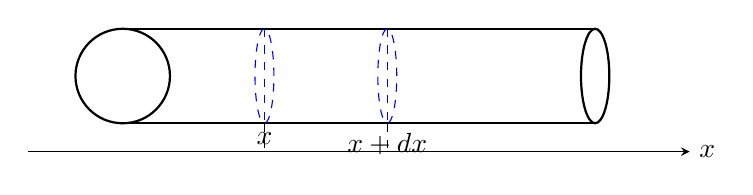
\begin{tikzpicture}[scale=1.2]
		% Cylinder
		\draw[thick] (0,0.5) -- (5,0.5);
		\draw[thick] (0,-0.5) -- (5,-0.5);
		\draw[thick] (0,0) circle (0.5);
		\draw[thick] (5,0) ellipse (0.15 and 0.5);
		
		% Segment [x, x+dx]
		\draw[dashed, blue] (1.5,0.5) -- (1.5,-0.5);
		\draw[dashed, blue] (1.5,0) ellipse (0.1 and 0.5);
		\node[below] at (1.5,-0.5) {$x$};
		
		\draw[dashed, blue] (2.8,0.5) -- (2.8,-0.5);
		\draw[dashed, blue] (2.8,0) ellipse (0.1 and 0.5);
		\node[below] at (2.8,-0.5) {$x+dx$};
		
		% Axis
		\draw[-stealth] (-1,-0.8) -- (6,-0.8) node[right] {$x$};
		\draw[dashed] (1.5,-0.5) -- (1.5,-0.8);
		\draw[dashed] (2.8,-0.5) -- (2.8,-0.8);
	\end{tikzpicture}
\end{center}

Введем обозначения:
\begin{itemize}
	\item $S$ --- площадь поперечного сечения стержня.
	\item $u(x,t)$ --- температура стержня в точке $x$ в момент времени $t$.
\end{itemize}

Если температура стержня распределена неравномерно, в нем возникают тепловые потоки. Согласно второму началу термодинамики, тепло передается от более горячих участков к более холодным.

\begin{theorem}{Закон Фурье}{fourier_law}
	Количество тепла, протекающее через поперечное сечение $x$ за промежуток времени $\Delta t$, пропорционально градиенту температуры и равно:
	\begin{equation}
		Q = q \cdot S \cdot \Delta t
	\end{equation}
	где плотность теплового потока $q$ определяется соотношением:
	\begin{equation}
		q = -k \cdot \pdv{u}{x}, \quad k > 0
	\end{equation}
	Величина $k$ называется коэффициентом теплопроводности, а $q$ представляет собой количество тепла, протекающее через единицу площади в единицу времени.
\end{theorem}

Вычислим количество тепла, полученное элементарным участком стержня $[x, x+dx]$ за время $\Delta t$ за счет теплопроводности:
\begin{equation}
	Q_{\text{приток}} = Q(x) - Q(x+dx) = k \cdot S \cdot \Delta t \qty( \eval{\pdv{u}{x}}_{x+dx} - \eval{\pdv{u}{x}}_{x} )
\end{equation}
Здесь $Q(x)$ --- тепло, вошедшее в элемент через левое сечение, а $Q(x+dx)$ --- тепло, ушедшее через правое сечение.

С другой стороны, количество тепла, необходимое для нагрева этого элементарного объема на величину $\Delta u$, равно:
\begin{equation}
	Q_{\text{нагрев}} = c \cdot m \cdot \Delta u = c \cdot \rho \cdot dx \cdot S \cdot \Delta u
\end{equation}
где:
\begin{itemize}
	\item $c$ --- удельная теплоемкость вещества стержня.
	\item $m = \rho \cdot dx \cdot S$ --- масса рассматриваемого элемента стержня.
	\item $\rho$ --- плотность вещества стержня.
\end{itemize}

Запишем уравнение теплового баланса ($Q_{\text{приток}} = Q_{\text{нагрев}}$):
\begin{equation}
	k \cdot S \cdot \Delta t \qty( \eval{\pdv{u}{x}}_{x+dx} - \eval{\pdv{u}{x}}_{x} ) = c \cdot \rho \cdot dx \cdot S \cdot \Delta u
\end{equation}
Разделим обе части на $c \cdot \rho \cdot dx \cdot S \cdot \Delta t$:
\begin{equation}
	\frac{k}{c \cdot \rho} \frac{\eval{\pdv{u}{x}}_{x+dx} - \eval{\pdv{u}{x}}_{x}}{dx} = \frac{\Delta u}{\Delta t}
\end{equation}

Переходя к пределу при $dx \to 0$ и $\Delta t \to 0$, получаем:
\begin{equation}
	\pdv{u}{t} = a^2 \pdv[2]{u}{x}, \quad \text{где } a^2 = \frac{k}{c \rho} > 0
\end{equation}
Данное уравнение называется \textbf{одномерным уравнением теплопроводности}, а параметр $a^2$ представляет собой коэффициент температуропроводности.

\begin{nb}
	Уравнение диффузии имеет абсолютно аналогичный вид, только вместо температуры $u(x,t)$ рассматривается концентрация диффундирующего вещества.
\end{nb}

\subsection{Метод Фурье для конечного стержня}

Рассмотрим однородный стержень длины $l$. Пусть его концы помещены в термостаты, температура которых поддерживается равной $0$.

\begin{center}
	\begin{tikzpicture}[scale=1]
		% Left thermostat
		\draw[pattern=north west lines, pattern color=gray] (-1,-0.8) rectangle (0,0.8);
		% Right thermostat
		\draw[pattern=north west lines, pattern color=gray] (4,-0.8) rectangle (5,0.8);
		% Rod
		\draw[thick] (0,0.4) -- (4,0.4);
		\draw[thick] (0,-0.4) -- (4,-0.4);
		\draw[thick] (0,0) ellipse (0.1 and 0.4);
		\draw[thick] (4,0) ellipse (0.1 and 0.4);
		
		\node at (-0.5,1.1) {Термостат $0^\circ$};
		\node at (4.5,1.1) {Термостат $0^\circ$};
		\node[below] at (2,-0.4) {Стержень длины $l$};
	\end{tikzpicture}
\end{center}

Математически задача формулируется в следующем виде:
\begin{equation}
	\begin{cases}
		\pdv{u}{t} = a^2 \pdv[2]{u}{x}, \quad 0 < x < l, \; t > 0 \quad &(1) \\
		u(x,0) = \varphi(x) \quad \text{-- начальное условие} \quad &(2) \\
		u(0,t) = u(l,t) = 0 \quad \text{-- краевые (граничные) условия} \quad &(3)
	\end{cases}
\end{equation}
Здесь $\varphi(x)$ задает начальное распределение температуры вдоль стержня.

Будем искать частные нетривиальные решения методом разделения переменных:
\begin{equation}
	u(x,t) = X(x) \cdot T(t) \quad (4)
\end{equation}
Подставляя (4) в исходное уравнение (1), получаем:
\begin{equation}
	X(x) \cdot T'(t) = a^2 X''(x) \cdot T(t) \iff \frac{T'(t)}{a^2 T(t)} = \frac{X''(x)}{X(x)} \quad (5)
\end{equation}
Так как левая часть зависит только от переменной $t$, а правая --- только от $x$, то равенство возможно лишь тогда, когда обе части равны постоянной константе $\lambda$:
\begin{equation}
	\frac{T'(t)}{a^2 T(t)} = \frac{X''(x)}{X(x)} = \lambda = \text{const} \quad (6)
\end{equation}

Отсюда получаем систему двух обыкновенных дифференциальных уравнений:
\begin{equation}
	\begin{cases}
		X'' - \lambda X = 0, \quad \text{где } X(x) \neq 0 \quad &(7) \\
		T' - \lambda a^2 T = 0, \quad \text{где } T(t) \neq 0 \quad &(8)
	\end{cases}
\end{equation}

Подставляя граничные условия (3), получаем:
\begin{equation}
	X(0) = X(l) = 0 \quad (9)
\end{equation}
Следовательно, для пространственной составляющей $X(x)$ имеем задачу на собственные значения:
\begin{equation}
	\begin{cases}
		X'' - \lambda X = 0 \\
		X(0) = X(l) = 0
	\end{cases} \quad (10)
\end{equation}

Рассмотрим три возможных случая для параметра $\lambda$:

\begin{example}[Случай 1: $\lambda > 0$]
	Пусть $\lambda = p^2$ ($p > 0$). Уравнение запишется как:
	\begin{equation}
		X'' - p^2 X = 0 \implies X(x) = A e^{-px} + B e^{px}
	\end{equation}
	Используем граничные условия (10):
	\begin{equation}
		\begin{cases}
			X(0) = A + B = 0 \implies B = -A \\
			X(l) = A e^{-pl} + B e^{pl} = 0 \implies A \qty( e^{-pl} - e^{pl} ) = 0
		\end{cases}
	\end{equation}
	Так как $p > 0$ и $l > 0$, разность $e^{-pl} - e^{pl} \neq 0$. Значит, $A=0$ и $B=0$, что дает тривиальное решение $X(x) \equiv 0$.
\end{example}

\begin{example}[Случай 2: $\lambda = 0$]
	Уравнение имеет вид $X'' = 0$. Общее решение:
	\begin{equation}
		X(x) = Ax + B
	\end{equation}
	Применяя граничные условия:
	\begin{equation}
		\begin{cases}
			X(0) = B = 0 \\
			X(l) = Al = 0 \implies A = 0
		\end{cases}
	\end{equation}
	Вновь получаем тривиальное решение $X(x) \equiv 0$.
\end{example}

\begin{example}[Случай 3: $\lambda < 0$]
	Пусть $\lambda = -p^2$ ($p > 0$). Уравнение Штурма-Лиувилля принимает вид:
	\begin{equation}
		X'' + p^2 X = 0 \implies X(x) = C \cos px + D \sin px \quad (11)
	\end{equation}
	Граничные условия дают:
	\begin{equation}
		\begin{cases}
			X(0) = C = 0 \\
			X(l) = D \sin pl = 0
		\end{cases}
	\end{equation}
	Для существования нетривиального решения необходимо положить $D \neq 0$. Отсюда следует:
	\begin{equation}
		\sin pl = 0 \implies pl = \pi n, \quad n \in \mathbb{Z} \implies p = \frac{\pi n}{l}
	\end{equation}
	Мы нашли собственные значения $\lambda_n$ и соответствующие им собственные функции $X_n(x)$:
	\begin{equation}
		\lambda_n = -\qty(\frac{\pi n}{l})^2, \quad X_n(x) = \sin \frac{\pi n}{l} x \quad (12)
	\end{equation}
	*(без потери общности положим константу $D$ равной $1$, так как она будет учтена при решении уравнения для $T(t)$).*
\end{example}

Теперь найдем решение для временной зависимости $T(t)$ из уравнения (8) при $\lambda = \lambda_n$:
\begin{equation}
	T' + \qty(\frac{\pi n}{l})^2 a^2 T = 0 \implies \frac{dT}{dt} = -p_n^2 a^2 T
\end{equation}
Разделяя переменные и интегрируя:
\begin{equation}
	\int \frac{dT}{T} = -p_n^2 a^2 \int dt \implies \ln|T| = -p_n^2 a^2 t + C \implies T_n(t) = A_n e^{-p_n^2 a^2 t} = A_n e^{-\qty(\frac{\pi n}{l})^2 a^2 t} \quad (13)
\end{equation}
где $A_n$ --- неопределенный коэффициент.

Перемножая пространственную и временную составляющие, получаем семейство частных решений, удовлетворяющих исходному уравнению и однородным краевым условиям:
\begin{equation}
	u_n(x,t) = X_n(x) \cdot T_n(t) = A_n e^{-\qty(\frac{\pi n}{l})^2 a^2 t} \sin \frac{\pi n}{l} x \quad (14)
\end{equation}

Для построения общего решения, удовлетворяющего произвольному начальному условию (2), воспользуемся принципом суперпозиции и представим решение в виде ряда Фурье:
\begin{equation}
	u(x,t) = \sum_{n=1}^{\infty} A_n e^{-\qty(\frac{\pi n}{l})^2 a^2 t} \sin \frac{\pi n x}{l} \quad (15)
\end{equation}

Коэффициенты $A_n$ определим, подставив начальное условие при $t=0$:
\begin{equation}
	u(x,0) = \sum_{n=1}^{\infty} A_n \sin \frac{\pi n x}{l} = \varphi(x) \quad (16)
\end{equation}
Коэффициенты этого разложения по ортогональной системе синусов вычисляются по формуле:
\begin{equation}
	A_n = \frac{2}{l} \int_0^l \varphi(x) \sin \frac{\pi n x}{l} dx \quad (17)
\end{equation}

Подставляя найденные коэффициенты (17) в ряд (15), получаем окончательное и единственное аналитическое решение поставленной начально-краевой задачи.

\subsection{Другие типы граничных условий}

\begin{enumerate}
	\item[1)] \textbf{Конечный теплоизолированный стержень (со всех сторон, включая торцы):}
	Если концы стержня также теплоизолированы, то тепловой поток через них равен нулю. Согласно закону Фурье, это эквивалентно равенству нулю производных температуры по координате на границах стержня:
	\begin{equation}
		\begin{cases}
			\pdv{u}{t} = a^2 \pdv[2]{u}{x} \quad &(18) \\
			u(x,0) = \varphi(x) \quad \text{-- начальное условие} \quad &(19) \\
			\eval{\pdv{u}{x}}_{x=0} = \eval{\pdv{u}{x}}_{x=l} = 0 \quad \text{-- краевые условия} \quad &(20)
		\end{cases}
	\end{equation}
	
	\item[2)] \textbf{Неоднородное уравнение теплопроводности:}
	Рассмотрим задачу при наличии внутренних источников или стоков тепла плотности $f(x,t)$ при однородных граничных условиях:
	\begin{equation}
		\begin{cases}
			\pdv{u}{t} = a^2 \pdv[2]{u}{x} + f(x,t), \quad 0 < x < l, \; t > 0 \quad &(27) \\
			u(x,0) = \varphi(x) \quad &(28) \\
			u(0,t) = u(l,t) = 0 \quad &(29)
		\end{cases}
	\end{equation}
	Решение данной задачи удобно представить в виде суммы двух функций:
	\begin{equation}
		u(x,t) = V(x,t) + W(x,t)
	\end{equation}
	где функции $V(x,t)$ и $W(x,t)$ определяются из двух вспомогательных систем:
	\begin{equation}
		\begin{cases}
			\pdv{V}{t} = a^2 \pdv[2]{V}{x} \\[1.5ex]
			V(x,0) = \varphi(x) \quad &(30) \\[1.5ex]
			V(0,t) = V(l,t) = 0
		\end{cases} \quad \text{и} \quad
		\begin{cases}
			\pdv{W}{t} = a^2 \pdv[2]{W}{x} + f(x,t) \\[1.5ex]
			W(x,0) = 0 \quad &(31) \\[1.5ex]
			W(0,t) = W(l,t) = 0
		\end{cases}
	\end{equation}
	
	\item[3)] \textbf{Уравнение теплопроводности с неоднородными краевыми условиями:}
	Если на границах стержня задан переменный во времени тепловой режим:
	\begin{equation}
		\begin{cases}
			\pdv{u}{t} = a^2 \pdv[2]{u}{x} \quad &(40) \\
			u(x,0) = \varphi(x) \quad &(41) \\
			\begin{aligned}
				u(0,t) &= \mu_1(t) \\
				u(l,t) &= \mu_2(t)
			\end{aligned} \quad \text{-- неоднородные краевые условия} \quad &(42)
		\end{cases}
	\end{equation}
\end{enumerate}
